In addition to running the \textit{DgsReduction} algorithm in Section~\ref{sec:Algs} directly, a graphical user interface (GUI) is also available, via the \textit{MantidPlot} analysis workbench. The GUI is launched from within \textit{MantidPlot} from the \textit{Interfaces} menu and selecting the \textit{DGS Reduction} menu entry. The GUI can also be used to export a Python script once the appropriate fields are filled for a reduction pass. The GUI also allows one to see the parameters outlined in Section~\ref{sec:Algs} that are read from the instrument parameter file. 

Once launched, the user is presented with the following layout (Figure~\ref{fig:SamSet}). The current instrument that is being requested for reduction is shown in the title bar of the GUI. To switch the reduction to a different instrument, use the \textit{Tools} menus and select the \textit{Change Instrument...} menu entry. 
\begin{figure}[ht]
\centerline{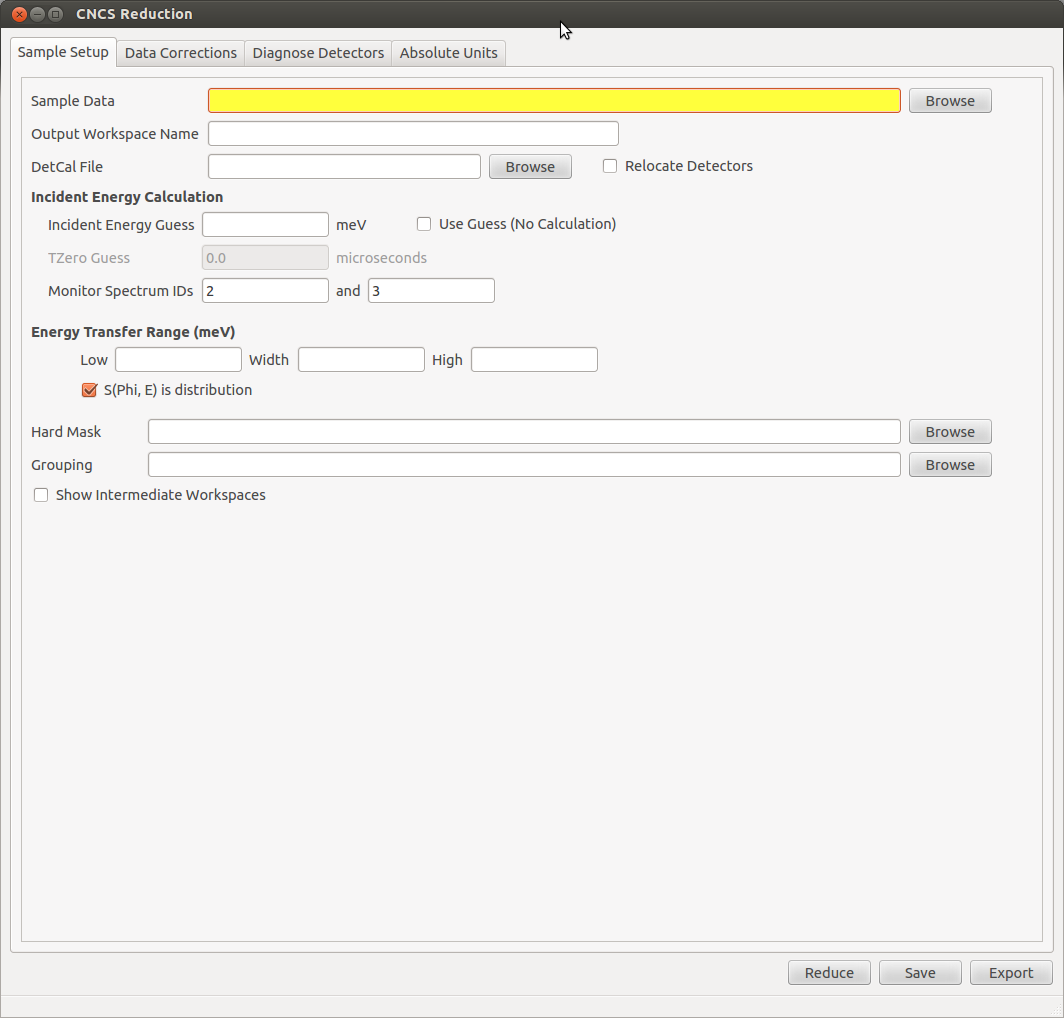
\includegraphics[width=0.75\textwidth]{figures/SampleSetup.png}}
\caption{Sample Setup tab on the DGS Reduction GUI}
\label{fig:SamSet}
\end{figure}
Besides the tab that shows up on launch, there are three (or four) other tabs for parameter entry. Each tab will be discussed individually in the next sections. To get start quickly, a reduction can be run with a minimal amount of information entered into the \textit{Sample Setup} tab. A file can be entered into the \textit{Sample Data} field. For \sns{} instruments, this is all that is required. \isis{} instruments will require an entry in the \textit{Incident Energy Guess} field in order to run. Once this minimal information is entered, the \textit{Reduce} button can be clicked to execute the reduction. On some computers, remote job submission is enabled. In that case a \textit{Send cluster} button appears, and can be used instead of the \textit{Reduce} one. More details are given in a later section. A Python script can be saved to a file by clicking the \textit{Export} button and filling in a file name to the subsequent dialog. A configuration file may be save by clicking the \textit{Save} button. This creates a XML file that can be loaded back into the GUI via the \textit{File/Open...} menu.
\subsection{Sample Setup}
As described earlier, the \textit{Sample Data} entry is the place to put a file (run) for reduction. The \textit{Browse} buttons allows you to locate that file via the standard file finder dialog. If this field is not filled in, the background color is yellow indicating that this field needs to be filled in before running reduction. The interface allows to reduce multiple files simultaneously, either separately or together, or even a combination of the two. For the syntax to use, see http://www.mantidproject.org/MultiFileLoading.

On certain computers with adequate privileges, a \textit{Use live stream} button appears for certain instruments. This allows on the fly reduction of the data, as it is collected.

The next field, \textit{Output Workspace Name}, allows you to control the name of the workspace as it appears in the \textit{MantidPlot} workspace listing. If nothing is entered, a default workspace name is created based on the sample file name without extension and the addition of this tag: '\_spe'. The \textit{DetCal File} entry is specific to \isis{} instruments. Under normal circumstances, the detector calibration file is just the input sample file, but this does not have to be the case. This entry can be used to point to a different detcal file for use in the reduction. The \textit{Relocate Detectors} checkbox controls a parameter that can relocate the detectors in the \textit{LoadDetectorInfo} \mantid{} algorithm that is run. 

Turning to the \textit{Incident Energy Calculation} section of the UI, the first entry field is \textit{Incident Energy Guess}. For \isis{} instruments, if no entry is made, the background color is yellow indicating this field needs to be filled in before running reduction. \sns{} instruments do not require an entry since the reduction algorithm will use the \textit{EnergyRequest} log to determine a guess. If a value is entered, then it will use that one instead of \textit{EnergyRequest}. If you wish to not have the reduction calculate the incident energy, but just use the value provided, you can check the \textit{Use Guess (No Calculation)} checkbox. Checking this option enables the \textit{TZero Guess} entry, which has a default value of zero microseconds and allows that parameter to be adjusted in accordance with the initial energy. The last set of entries deals with the \textit{Monitor Spectrum IDs} used to perform the initial energy calculation. These two values are read from the instrument parameter file, so by default this is what the reduction algorithm uses. The entries allow you to override the IDs in order to use different monitors to perform the calculation. For the \sns{} instruments, CNCS and HYSPEC, the \textit{Incident Energy Guess} is automatically used as the incident energy, and the time zero value is calculated via a formula found in the instrument parameter file.

The next section is the \textit{Energy Transfer Range} entries. The first three entries allow you to specify the binning strategy for the x-axis of the output $S(\theta, \phi, E)$. If no values are entered, a default binning strategy is constructed by the reduction algorithm. Using the initial energy guess, $E^{guess}_i$, the low, width and high values are $-0.5E^{guess}_i$, $0.01E^{guess}_i$, $0.99E^{guess}_i$. If you want to fill in values, all the entries must be filled. The last option is the \textit{S(Phi, E) is distribution} checkbox. This option causes the resulting data to be converted to a $\frac{d^2\sigma(\theta,\phi,E)}{dE d\Omega}$ or $S(\theta, \phi, E)$ histogram workspace by dividing by the bin width from the x-axis binning. Disabling this option stops this division and will keep an event workspace as the final result if the input was an event workspace and no time-independent background subtraction was requested. 

The first of the last set of options allows one to apply a hard mask to the data by setting a file in the \textit{Hard Mask} entry. A grouping file (sometimes know as a mapping file) which aggregates data into large blocks can be applied to the data by setting a file in the \textit{Grouping} entry. The \textit{Show Intermediate Workspaces} can be used to display workspaces created during the reduction process in addition to the output workspace. 

Processed \nexus{} files are saved for each set of files added together in the directory specified by \textit{Save to folder}. No files are saved for live reduction. In case of remote cluster submission, users should not specify folders where the cluster cannot write output files.


\subsection{Data Corrections}
This tab (Figure~\ref{fig:DataCorr}) deals with corrections that are applied to the sample data. The first set of entries deals with the \textit{Incident Beam Normalisation}. This group of radio buttons allows one to pick the type of incident beam normalisation to perform. The default, \textit{None}, performs no normalisation on the data. The \textit{Current} option divides the data by its corresponding value of the proton charge. The \textit{Monitor 1} option uses the monitor specified in the instrument parameter file to integrate the time-of-flight range given in the \textit{Integration Range} entries. The values in these entries are also read from the instrument parameter file. The radio buttons enforce that only one type of incident beam monitor normalisation can be performed on all input datasets.

\begin{figure}[ht]
\centerline{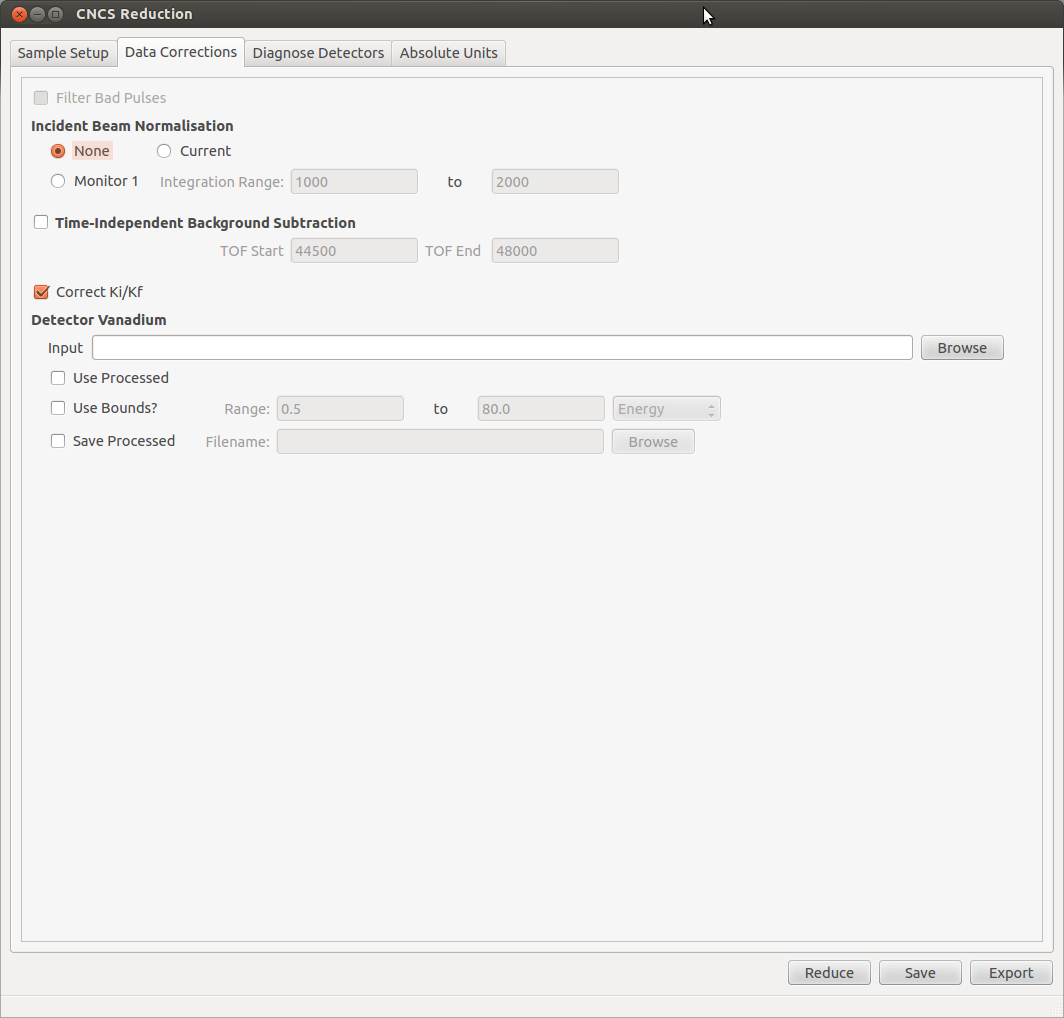
\includegraphics[width=0.75\textwidth]{figures/DataCorrections.png}}
\caption{Data Corrections tab on the DGS Reduction GUI}
\label{fig:DataCorr}
\end{figure}

The next section is deals with the \textit{Time-Independent Background Subtraction} parameters. Here, the two entries represent the time-of-flight range in between which the background value will be determined. These parameters are also read from the instrument parameter file. The determined background will then be subtracted from the sample workspace. 

The \textit{Correct Ki/Kf} converts $\frac{d^2\sigma(\theta,\phi,E)}{dE d\Omega}$ to $S(\theta, \phi, E)$ and is applied by default. 

The last section deals with the \textit{Detector Vanadium} that is associated with the sample input data. The \textit{Input} entry is where you can input a detector vanadium file (run) for use in the reduction. The \textit{Browse} button will allow you to search for the file via the normal file dialog. The \textit{Incident Beam Normalisation} chosen earlier will be applied if you do not use a pre-processed file. The \textit{Use Processed} checkbox allows you to tell the reduction that the file you are providing has already been processed and just needs to be used as is in the reduction. How you save a processed detector vanadium will be covered soon. If \textit{Used Processed} is checked, all the following entries are cleared and disabled. Otherwise, the detector vanadium is processed according to the procedure in Section~\ref{sec:Algs}. The data is integrated according to the integration range given in the instrument parameter file. However, you can request alternative bounds by checking the \textit{Use Bounds?} checkbox. This activates the \textit{Range} entries, in which you can specify the bounds of the integration for the detector vanadium. The units on the bounds are assumed to be energy in the instrument parameter file. You can use the combobox at the end of the \textit{Range} entries to set the units on the integration bounds. The available options are Energy, Wavelength and TOF (time-of-flight). Setting the units to anything other than time-of-flight will cause a unit conversion to occur on the detector vanadium data. The last options are used for if you are processing the detector vanadium for the first time. Checking the \textit{Save Processed} checkbox allows you to save a \nexus{} file containing the processed detector vanadium. Using this checkbox activates the Filename entry so that you can provide an output file name for the saved file. If you do not put anything into the entry, a default file name will be created and looks like ``\textit{\textless OutputWorkspaceName \textgreater}\_idetvan.nxs" and the file will be saved in the \mantid{} default output directory. 
\subsection{Diagnose Detectors}\label{sec:UI-DiagDet}
This tab (Figure~\ref{fig:DiagDet}) deals with performing diagnostic tests on the detector vanadium data being used in the reduction as well as the sample data for the reduction. On this tab, almost all of the entries and checkbox states are read from the instrument parameter file. The only exception is the \textit{Detector Van 2} entry. These parameters are the ones that the reduction algorithm will use in the diagnostic tests unless the values are changed in the GUI. 

\begin{figure}[ht]
\centerline{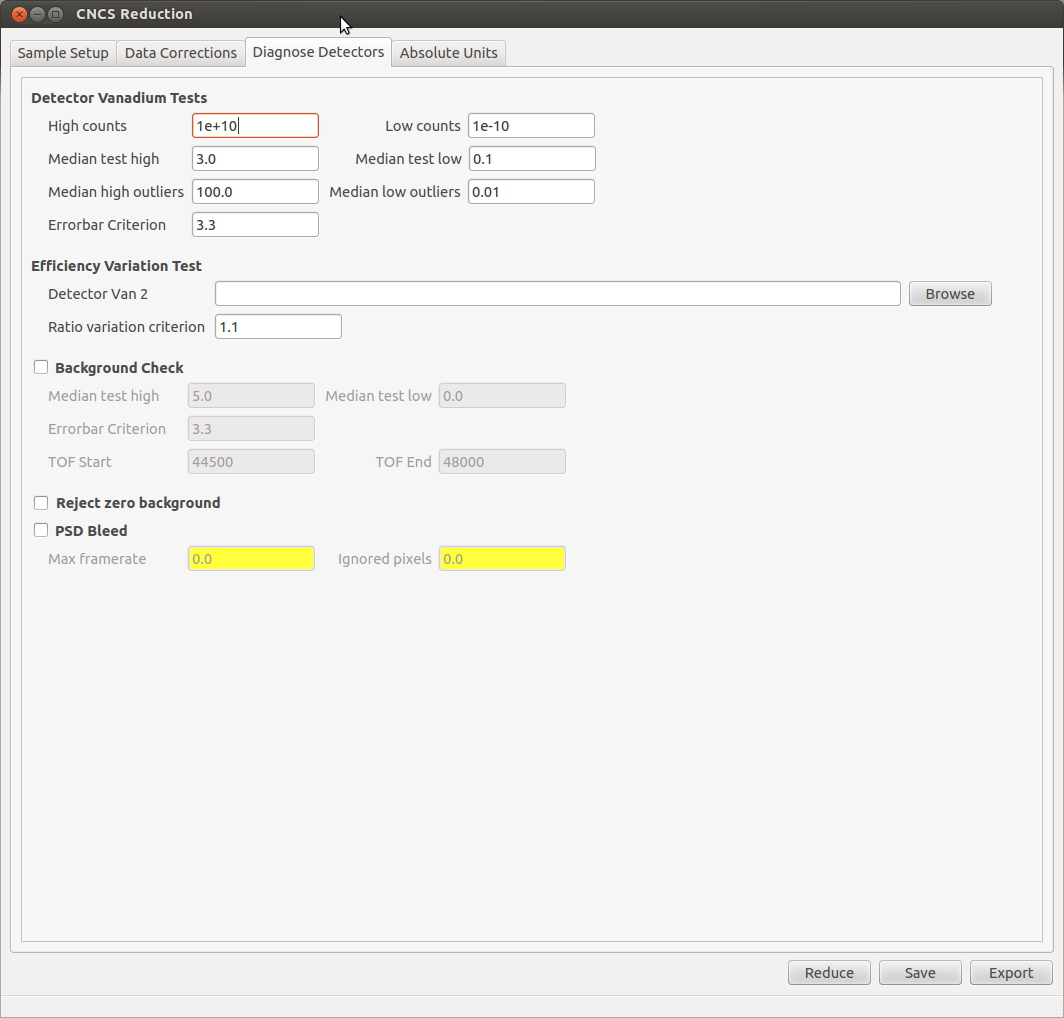
\includegraphics[width=0.75\textwidth]{figures/DiagnoseDetectors.png}}
\caption{Diagnose Detectors tab on the DGS Reduction GUI}
\label{fig:DiagDet}
\end{figure}

The first section, \textit{Detector Vanadium Tests}, deals with the parameters used for the two tests (\textit{FindDetectorsOutsideLimits} and \textit{MedianDetectorTest}) run on the detector vanadium data, which may already have a hard mask applied. All of the parameters in this section are read from the instrument parameter file. The \textit{High counts} and \textit{Low counts} parameters are used in the \textit{FindDetectorsOutsideLimits} algorithm to determine hot and cold pixels in the data. All of the other parameters in this section are used in the \textit{MedianDetectorTest} algorithm. Once the median is calculated, the \textit{Median high outliers} and \textit{Median low outliers} entries are used as multipliers on the median and any pixel outside the bounds is masked and then the median is recalculated. Next, the \textit{Median test high} and \textit{Median test low} are used as multipliers on the median and any pixel outside the bounds is masked. The \textit{Errorbar Criterion} entry is used in conjunction with previous two parameters, but checks the pixel signal minus the median.

The \textit{Efficiency Variation Test} section uses a second set of detector vanadium data to compare against the original detector vanadium data. The \textit{Detector Van 2} entry is where you specify this second detector vanadium file (run). The \textit{Browse} button can help you find a file via the normal dialog. The \textit{Ratio variation criterion} entry is the parameter used to check the consistency between the two detector vanadium datasets. This is used by the \textit{DetectorEfficiencyVariation} test which is run after the two previously described tests are run on the second detector vanadium.

The \textit{Background Check} checkbox activates the parameters below it and will perform a \textit{MedianDetectorTest} on a sample workspace that has been incident beam normalised and integrated over the background range given by the \textit{TOF Start} and \textit{TOF End} entry parameters. The other parameters are just in conjunction with the \textit{MedianDetectorTest} are are described previously. All the parameters in this section are read from the instrument parameter file.

The \textit{Reject zero background} checkbox activates a \textit{FindDetectorsOutsideLimits} test on a sample workspace that has been incident beam normalised and integrated over the entire range of data present (one number per detector pixel or total counts). This test is hard-wired to check for detector pixels having their total counts between $1\times10^{-10}$ and $1\times10^{100}$. 

The \textit{PSD Bleed} checkbox triggers the activation of the \textit{CreatePSDBleedMask} test.
This test uses the \textit{Max Framerate} and \textit{Ignored pixels} parameters to determine which tubes are counting above the maximum frame rate. These tubes will be masked if they fail this check. The ignored pixels parameter tells how many pixels around the central region are ignored in the check.
\subsection{Absolute Units}
This tab (Figure~\ref{fig:AbsUnits}) handles collecting the data and parameters for calculating the absolute units normalisation data. Checking the \textit{Perform Absolute Normalisation} checkbox will activate this reduction procedure. 

\begin{figure}[ht]
\centerline{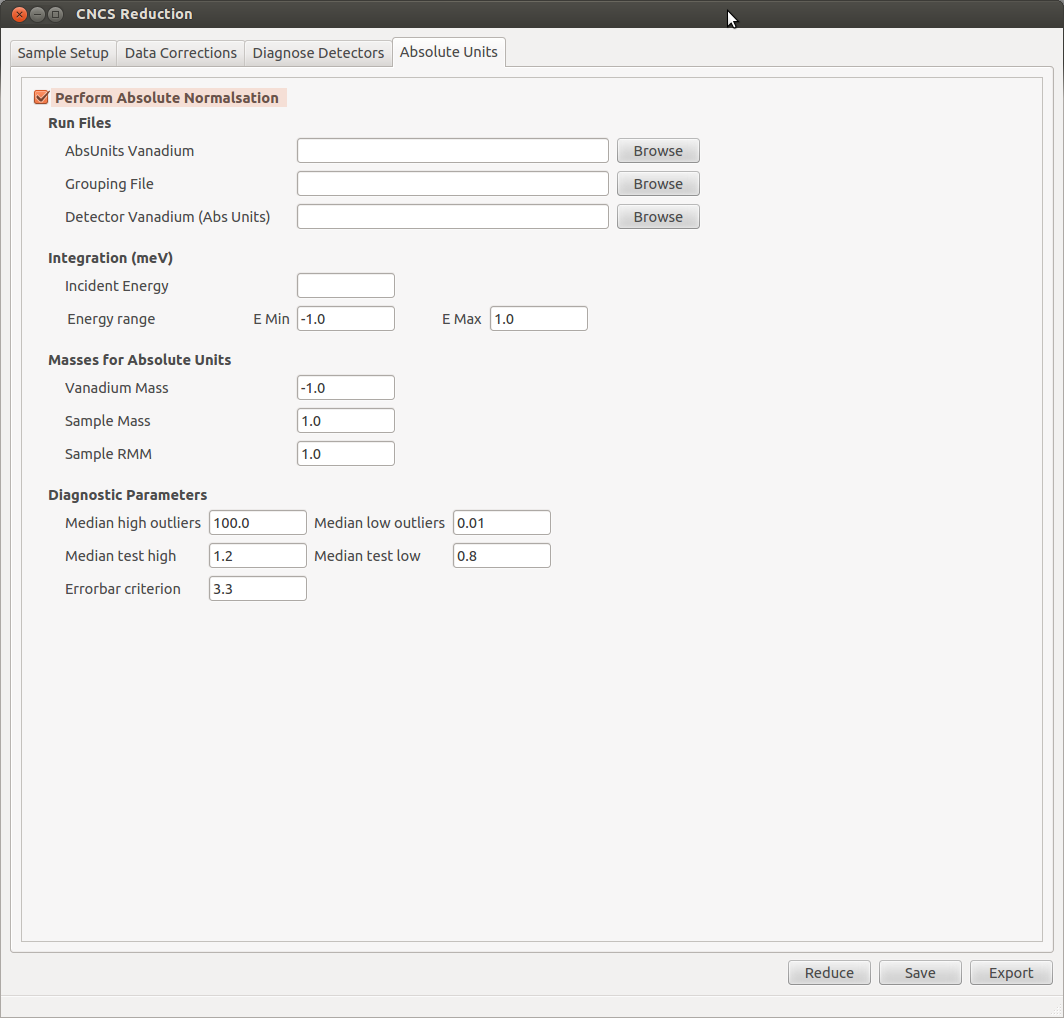
\includegraphics[width=0.75\textwidth]{figures/AbsoluteUnits.png}}
\caption{Absolute Units tab on the DGS Reduction GUI}
\label{fig:AbsUnits}
\end{figure}

The first section, \textit{Run Files}, handles setting the appropriate data files for the absolute units calculation. The \textit{AbsUnits Vanadium} entry allows you to set the appropriate file (run) containing the absolute units sample data. As usual, the \textit{Browse} button can be used to navigate to a file. The \textit{Grouping File} entry allows you to group (map) the absolute units sample data during processing. This grouping is usually the same as the sample and sample detector vanadium processing, but this is not enforced. The \textit{Detector Vanadium (AbsUnits)} entry allows you to specify a detector vanadium for the absolute units processing. Again, this detector vanadium is usually the one used for the sample data, but does not have to be. 

The next section, \textit{Integration}, deals with setting the parameters for the integration of the absolute units sample data. The \textit{Incident Energy} entry allows you to specify the incident energy for the absolute units sample data. This is usually the same as the incident energy for the sample data, but does not necessarily have to be. The \textit{EMin} and \textit{EMax} entries for the \textit{Energy Range} are where you specify the range over which to accumulate the values that will go into the final value for the absolute units normalisation. These two parameters are read from the instrument parameter file.

The following section, \textit{Masses for Absolute Units}, manages setting constants that will be applied to the final absolute units normalisation result. The \textit{Vanadium Mass} entry is where you specify the amount of vanadium (in grams) used as the absolute unit sample. This parameter is read from the instrument parameter file and if a $-1.0$ is shown, no good value is provided in the file. Since the absolute units is applied against the sample data, the number of moles of sample is calculated via the ratio of the \textit{Sample Mass} and \textit{Sample RMM} parameters. The first entry is the amount of the sample (in grams) being used and the second entry is the relative molecular mass of the sample. The default for both parameters is $1.0$ which means there is no a priori knowledge of the sample data. For calculation of the number of moles of Vanadium, the atomic mass is hard-coded and the \textit{Vanadium Mass} parameter is used.

The last section, \textit{Diagnostic Parameters}, handles setting the quantities used in the same diagnostic tests that were discussed in Section~\ref{sec:UI-DiagDet}. In this case, only the \textit{FindDetectorsOutsideLimits} and \textit{MedianDetectorTest} are run on the absolute units sample after detector vanadium correction (if applicable). All of the parameters in this section are read from the instrument parameter file.

\subsection{Remote jobs}

\begin{figure}[ht]
\centerline{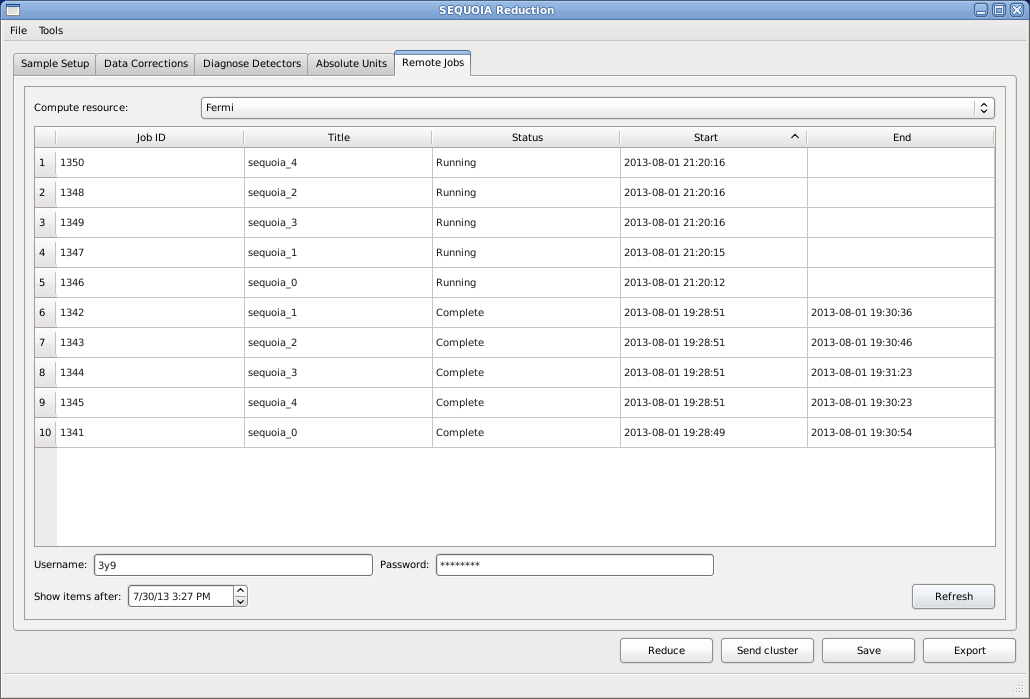
\includegraphics[width=0.75\textwidth]{figures/cluster.png}}
\caption{Remote jobs tab on the DGS Reduction GUI}
\label{fig:cluster}
\end{figure}

The \textit{DGS Reduction} interface allows submission of jobs in parallel to compute clusters (currently only Fermi at ORNL). One job is created for each set of files that are added together. On first \textit{Send cluster} use, the user is prompted to select number of nodes and cores, and to provide username and password. Once the jobs are submitted, one can check the status in the \textit{Remote jobs} tab (Figure \ref{fig:cluster}). User can select the most recent jobs by setting the value for \textit{Show items after} and clicking the \textit{Refresh} button. 

